\begin{frame}
\frametitle{HES: Hypertext Editing System}
\begin{itemize}
	\item 1967
	\item Andries van Dam and Ted Nelson, Brown University
	\item IBM/360 Model 50 Mainframe
	\item Dokumentation der Apollo Missionen, NASA
\end{itemize}

\begin{figure}[htbp]
	\centering
	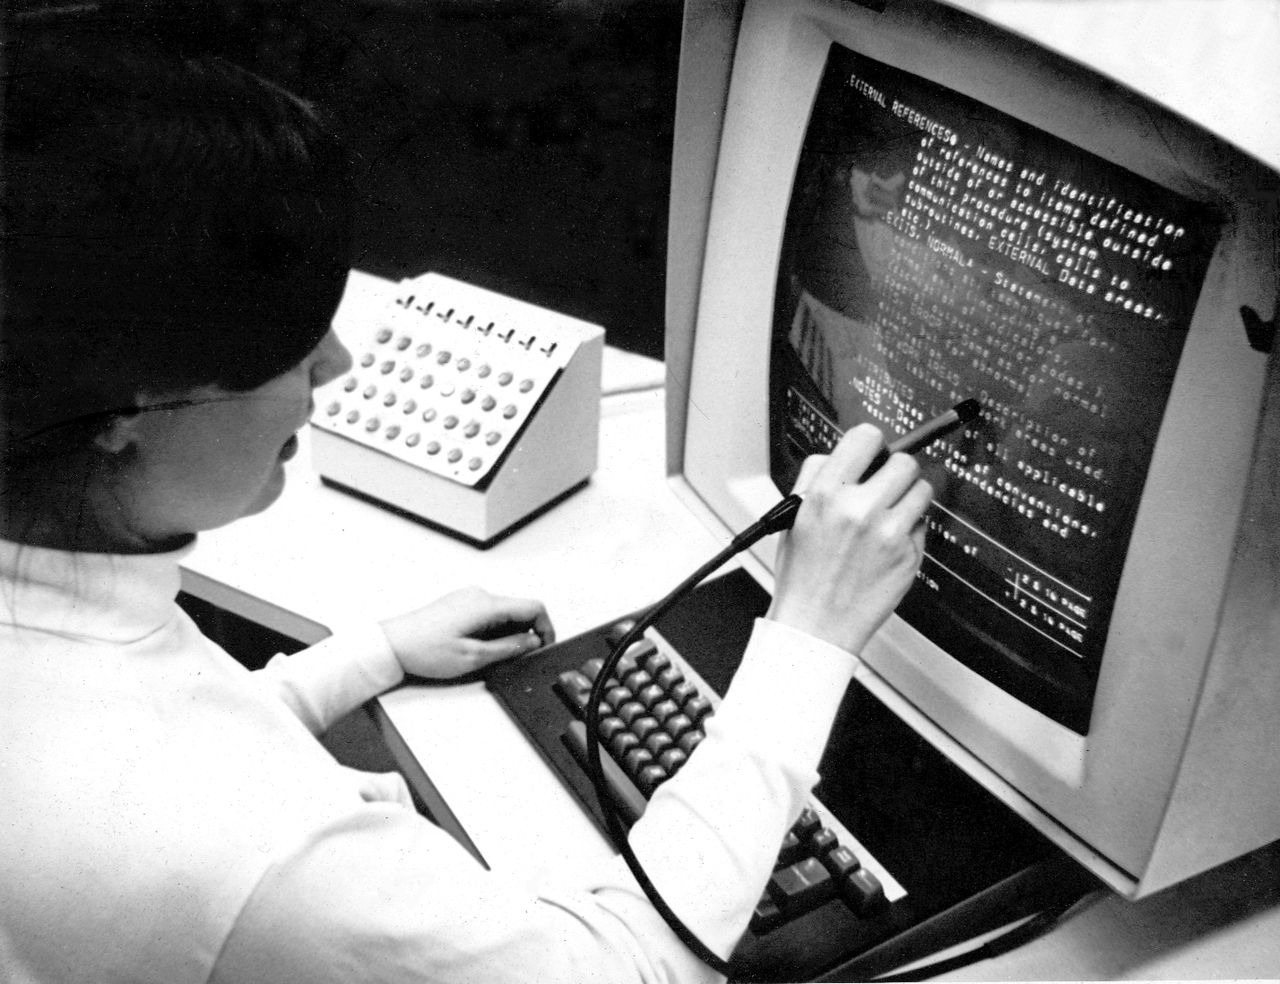
\includegraphics[width=0.40\textwidth]{images/hes}
\end{figure}

\end{frame}

\begin{frame}
\frametitle{HES: Hypertext Editing System}
\framesubtitle{Funktionen}
	\begin{itemize}
		\item Userinterface / Bedienmöglichkeiten
		\begin{itemize}
			\item Lightpenning und Tastatur
			\item Graph Darstellung
		\end{itemize}
		\item Links / Strukturen
		\begin{itemize}
			\item Kontrollinformationen für eine lineare Darstellung
			\item Pointer zu Text Fragmenten
			\item Textpassagen mit Labels referenzierbar
		\end{itemize}
	\end{itemize}
\end{frame}

\begin{frame}
\frametitle{FRESS: File Retrieval and Editing System}
\framesubtitle{Funktionen}
\begin{itemize}
	\item 1968
	\item Andries van Dam, Bob Wallace und Studenten
	\item Kommerzielle Betriebssysteme
	\item Weiterentwicklung von HES
	\item Userinterface / Bedienmöglichkeiten
	\begin{itemize}
		\item Backtrack durch die Links
		\item Windows
		\item UNDO Feature
		\item auf PDS-1 (Minicomputer): Light Pen und Fußpedal
	\end{itemize}
	\item Links / Strukturen
	\begin{itemize}
		\item one-way Links (tag)
		\item bi-direktionale Links (jumps)
		\item unbegrenzte Dokumentgrößen
	\end{itemize}
\end{itemize}
\end{frame}
